\section{Auswertung}
\label{sec:Auswertung}

% Abmessungen Acrylblock
\subsection{Abmessungen des Acrylblocks}
\label{sec:Abmessungen}
Die Höhe des Acrylblocks wird zu
\begin{equation*}
    h = \qty{80,5}{\milli\metre}
\end{equation*}
bestimmt. Aus der Höhe und den Abständen der Bohrungen zu der oberen und der unteren Kante wird außerdem der Durchmesser berechnet.
\begin{table}[H]
    \centering
    \caption{Abmessungen des Acrylblocks.}
    \label{tab:Schieblehre}
    \begin{tabular}{S[table-format=2.0] S[table-format=2.1] S[table-format=2.1] S[table-format=2.1]}
        \toprule
         {Lochnummer} & {$s_{\symup{oben}}\,/\,\unit{\milli\metre}$} & {$s_{\symup{unten}}\,/\,\unit{\milli\metre}$} %
         & {$d\,/\,\unit{\milli\metre}$}\\
        \midrule
         1	& 13.1	& 61.3 &  6.1 \\
         2	& 21.7	& 53.9 &  4.9 \\
         3	& 30.2	& 46.3 &  4.0 \\
         4	& 38.8	& 39.0 &  2.7 \\
         5	& 46.6	& 31.0 &  2.9 \\
         6	& 54.8	& 23.0 &  2.7 \\
         7	& 63.6	& 15.0 &  1.9 \\
         8	& 70.5	&  7.0 &  3.0 \\
         9	& 10.3	& 55.4 & 14.8 \\
         10	& 59.6	& 19.5 &  1.4 \\
         11	& 61.3	& 17.9 &  1.3 \\
        \bottomrule 
    \end{tabular}
  \end{table}

% c_Acryl
\subsection{Bestimmung der Schallgeschwindigkeit in Acryl}
Aus der Laufzeit der Ultraschallwellen und der aus \ref{sec:Abmessungen} bekannten Positionen der Bohrungen wird ein Plot erstellt. Mithilfe einer 
linearen Ausgleichsrechnung mit der \textit{python}-Erweiterung \textit{scipy} \cite{scipy} wird eine Regressiongerade vom Typ $y=mx+b$ mit den
Parametern
\begin{align*}
    m &= \qty{360.3(3.0)e-6}{\second\per\metre} \\
    b &= \qty{0.7(3.0)e-6}{\second}
\end{align*}
bestimmt. Aus \eqref{eq:Impuls-Echo} wird die Schallgeschwindigkeit in Acryl zu
\begin{equation*}
    c_{\symup{exp}} = \frac{1}{m} = \qty{2775+-23}{\metre\per\second}
\end{equation*}
berechnet. Der Parameter $b$ beschreibt die Laufzeit des Schallimpules in der Kopplungsschicht. Mit der Schallgeschwindigkeit in der Kopplungsschicht
von $c_{\symup{Wasser}} = \qty{1483}{\metre\per\second}$ \cite{czichos} kann die Dicke der Kopplungsschicht $\tilde{d_{\symup{K}}}$ bestimmt werden.
\begin{equation*}
    \tilde{d}_{\symup{K}} = c_{\symup{Wasser}} \cdot b = \qty{1+-4}{\milli\metre}
\end{equation*}

\begin{table}[H]
    \centering
    \caption{Daten $c$-Bestimmung mit Impuls-Echo-Verfahren.}
    \label{tab:c-bestimmung}
    \begin{tabular}{S[table-format=1.0] S[table-format=2.1] S[table-format=2.1]}
        \toprule
         {Lochnummer} & {$s_{\symup{oben}}\,/\,\unit{\milli\metre}$} & {$\symup{\Delta}t\,/\,\unit{\micro\second}$} \\
        \midrule
         1	& 13,1	& 10,7 \\
         2	& 21,7	& 16,9 \\
         3	& 30,2	& 23,1 \\
         4	& 38,8	& 29,5 \\
         5	& 46,6	& 35,3 \\
         6	& 54,8	& 41,0 \\
         7	& 63,6	& 46,8 \\ 
        \bottomrule 
    \end{tabular}
  \end{table}

\begin{figure}[H]
    \centering
    \includegraphics{c-bestimmung.pdf}
    \caption{Graphische Darstellung der Messwertpaare aus \autoref{tab:c-bestimmung} mit Ausgleichsgerade.}
    \label{fig:c-bestimmung}
  \end{figure}

% Dicke Kopplungsschicht
\subsection{Berechnung der Dicke der Kopplungsschicht}
Die aus der linearen Regression bestimmte Dicke der Kopplungsschicht weist eine große Messunsicherheit auf, weshalb hier mit einer anderen
Berechnungsmethode versucht wird, diese Unsicherheit zu verringern.

Dafür wird der aus \ref{sec:Abmessungen} bekannte Abstand der Bohrungen zur Oberkante und ein Literaturwert für die Schallgeschwindigkeit
in Acryl von $c_{\symup{Acryl}} = \qty{2730}{\metre\per\second}$ \cite{c_Acryl} verwendet, um so die theoretische Laufzeit des Schallimpules 
zu berechnen. Aus der Differenz der tatsächlichen und der theoretischen Laufzeit aus \autoref{tab:c-bestimmung} kann so wieder mit der 
Schallgeschwindigkeit in der Kopplungsschicht die Dicke dieser zu
\begin{equation*}
    d_{\symup{K}} = \qty{0.68+-0.22}{\milli\metre}
\end{equation*}
bestimmt werden.

Im Folgenden wird aufrund der geringeren Messunsicherheit dieser Wert verwendet.

% Vermessung mit A-Scan
\subsection{Vermessung des Acrylzylinder mit einem A-Scan}
\label{sec:a-scan}
Die Abstände der Bohrungen zu der oberen und unteren Seite des Acrylblocks müssen um die Dicke der Anpassungsschicht korrigiert werden. 
Zur Veranschaulichung wird außerdem die relative Abweichung der korrigierten Messwerte zu den Werten aus \ref{sec:Abmessungen} angegeben.

  \begin{table}[H]
    \centering
    \caption{Unkorrigierte Daten der Vermessung des Acrylblocks mit einem A-Scan.}
    \label{tab:a-scan}
    \begin{tabular}{S[table-format=2.0] S[table-format=2.1] S[table-format=2.1] S[table-format=2.1]}
        \toprule
         {Lochnummer} & {$\tilde{s}_{\symup{oben}}\,/\,\unit{\milli\metre}$} & {$\tilde{s}_{\symup{unten}}\,/\,\unit{\milli\metre}$} \\
        \midrule
         1	& 14.7 & 62.5 \\
         2	& 23.1 & 55.1 \\
         3	& 31.6 & 47.6 \\
         4	& 40.0 & 40.2 \\
         5	& 48.1 & 32.2 \\
         6	& 56.0 & 24.1 \\
         7	& 63.9 & 16.3 \\
         8	& 72.3 &  8.4 \\
         9	& 16.6 & 56.7 \\
         10	& 60.7 & 20.7 \\
         11	& 62.4 & 19.2 \\
        \bottomrule 
    \end{tabular}
  \end{table}

  \begin{table}[H]
    \centering
    \caption{Korrigierte Daten der Vermessung des Acrylblocks mit einem A-Scan.}
    \label{tab:a-scan_korr}
    \begin{tabular}{S[table-format=2.0] S[table-format=2.1] S[table-format=2.2] S[table-format=2.1] S[table-format=1.2]}
        \toprule
         {Lochnummer} & {$s_{\symup{oben}}\,/\,\unit{\milli\metre}$} & {$\symup{\Delta}_{\symup{rel}}(s_{\symup{oben}})\,/\,\unit{\percent}$} & %
         {$s_{\symup{unten}}\,/\,\unit{\milli\metre}$} & {$\symup{\Delta}_{\symup{rel}}(s_{\symup{unten}})\,/\,\unit{\percent}$} \\
        \midrule
         1	& 13.3 &  1.90 & 61.1 & 0.25 \\
         2	& 21.7 &  0.23 & 53.7 & 0.28 \\
         3	& 30.2 &  0.16 & 46.2 & 0.11 \\
         4	& 38.6 &  0.39 & 38.8 & 0.39 \\
         5	& 46.7 &  0.32 & 30.8 & 0.49 \\
         6	& 54.6 &  0.28 & 22.7 & 1.09 \\
         7	& 62.5 &  1.65 & 14.9 & 0.34 \\
         8	& 70.9 &  0.64 &  7.0 & 0.70 \\
         9	& 15.2 & 48.05 & 55.3 & 0.09 \\
         10	& 59.3 &  0.42 & 19.3 & 0.77 \\
         11	& 61.0 &  0.41 & 17.8 & 0.28 \\
        \bottomrule 
    \end{tabular}
  \end{table}

% Untersuchung des Auflösungsvermögen
\subsection{Untersuchung des Auflösungsvermögen}
Die Bohrungen 10 und 11 werden von der unteren Seite aus mit den beiden Messsonden betrachtet.
\begin{figure}
    \begin{subfigure}{0.48\textwidth}
      \centering
      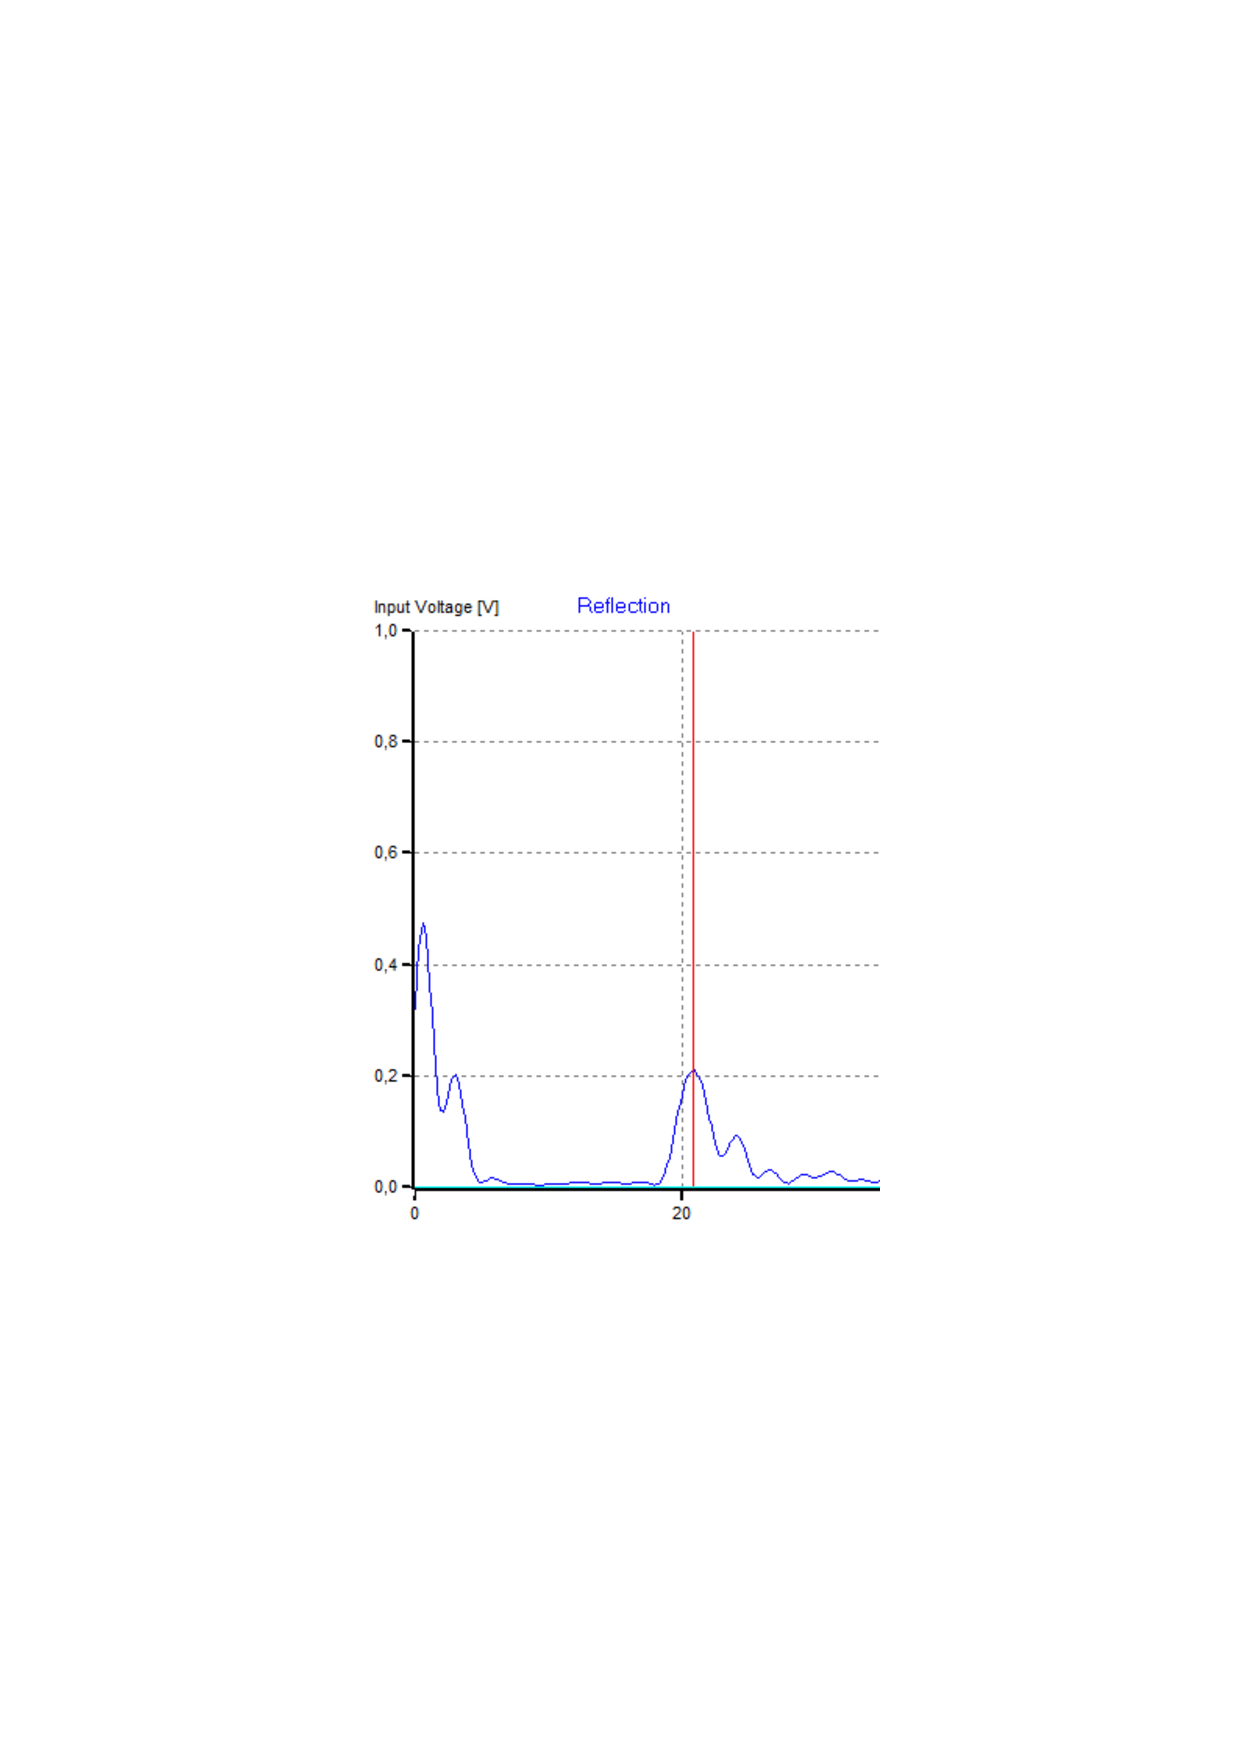
\includegraphics[height=5cm]{content/pics/1MHz.pdf}
      \caption{1\,MHz-Messsonde}
      \label{fig:1MHz}
    \end{subfigure}
    \hfill
    \begin{subfigure}{0.48\textwidth}
      \centering
      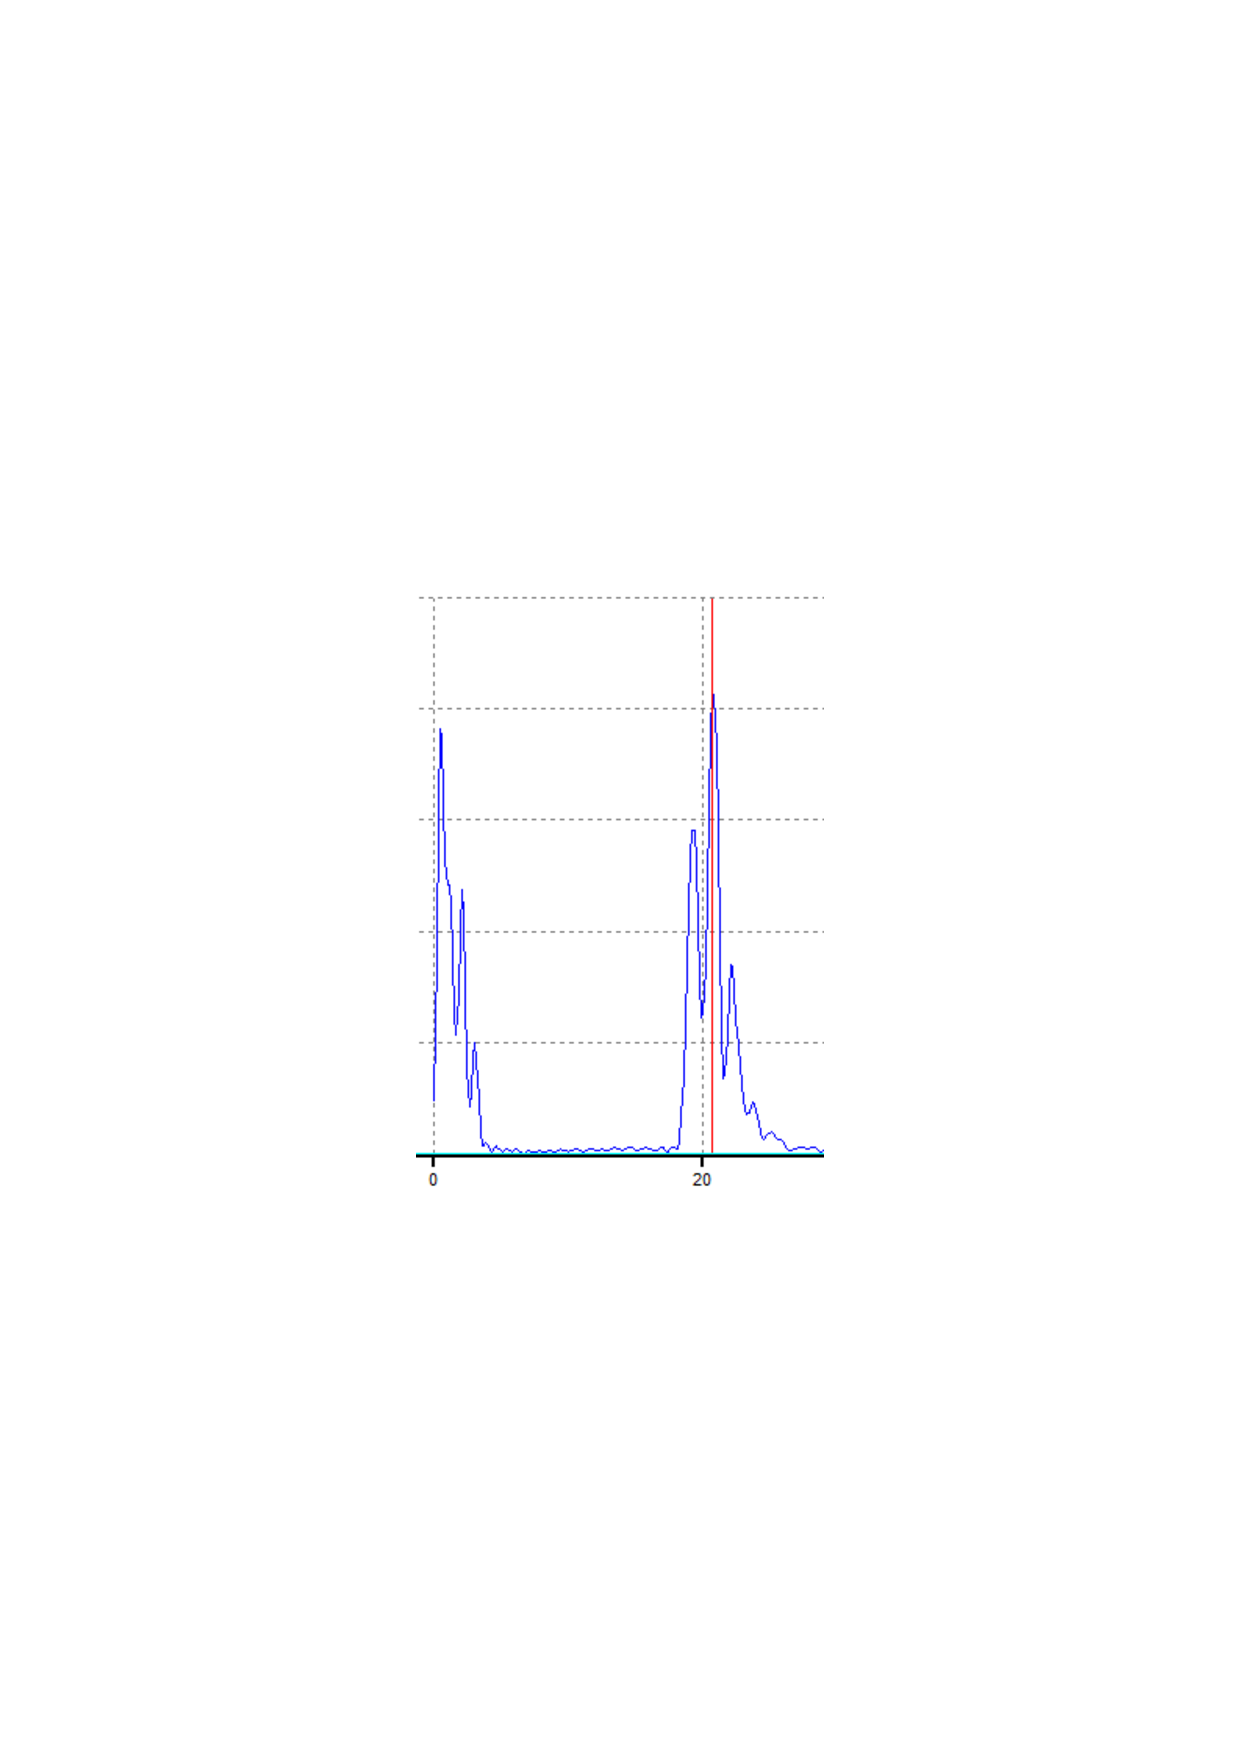
\includegraphics[height=5cm]{content/pics/2MHz.pdf}
      \caption{2\,MHz Messonde}
      \label{fig:2MHz}
    \end{subfigure}
    \caption{Ausgabe eines A-Scans der Bohrungen 10 und 11 mit verschiedenen Messsonden.}
    \label{fig:Auflösung}
  \end{figure}
Es ist zu erkennen, dass mit der $\qty{2}{\mega\hertz}$ Sonde deutlich besser zwischen den beiden nah aneinanderliegenden distinguiert 
werden kann. Die Breite der Peaks ist bei der $\qty{2}{\mega\hertz}$ Sonde geringer als die der anderen Sonde, was das exakte Ablesen der
Tiefe der Bohrungen erleichtert.

% Vermessung mit B-Scan
\subsection{Vermessung des Acrylzylinder mit einem B-Scan}
Aus den Graphiken der B-Scans der oberen und unteren Seite werden wie in \ref{sec:a-scan} die Tiefen der Bohrungen abgelesen.

\begin{figure}[H]
    \centering
    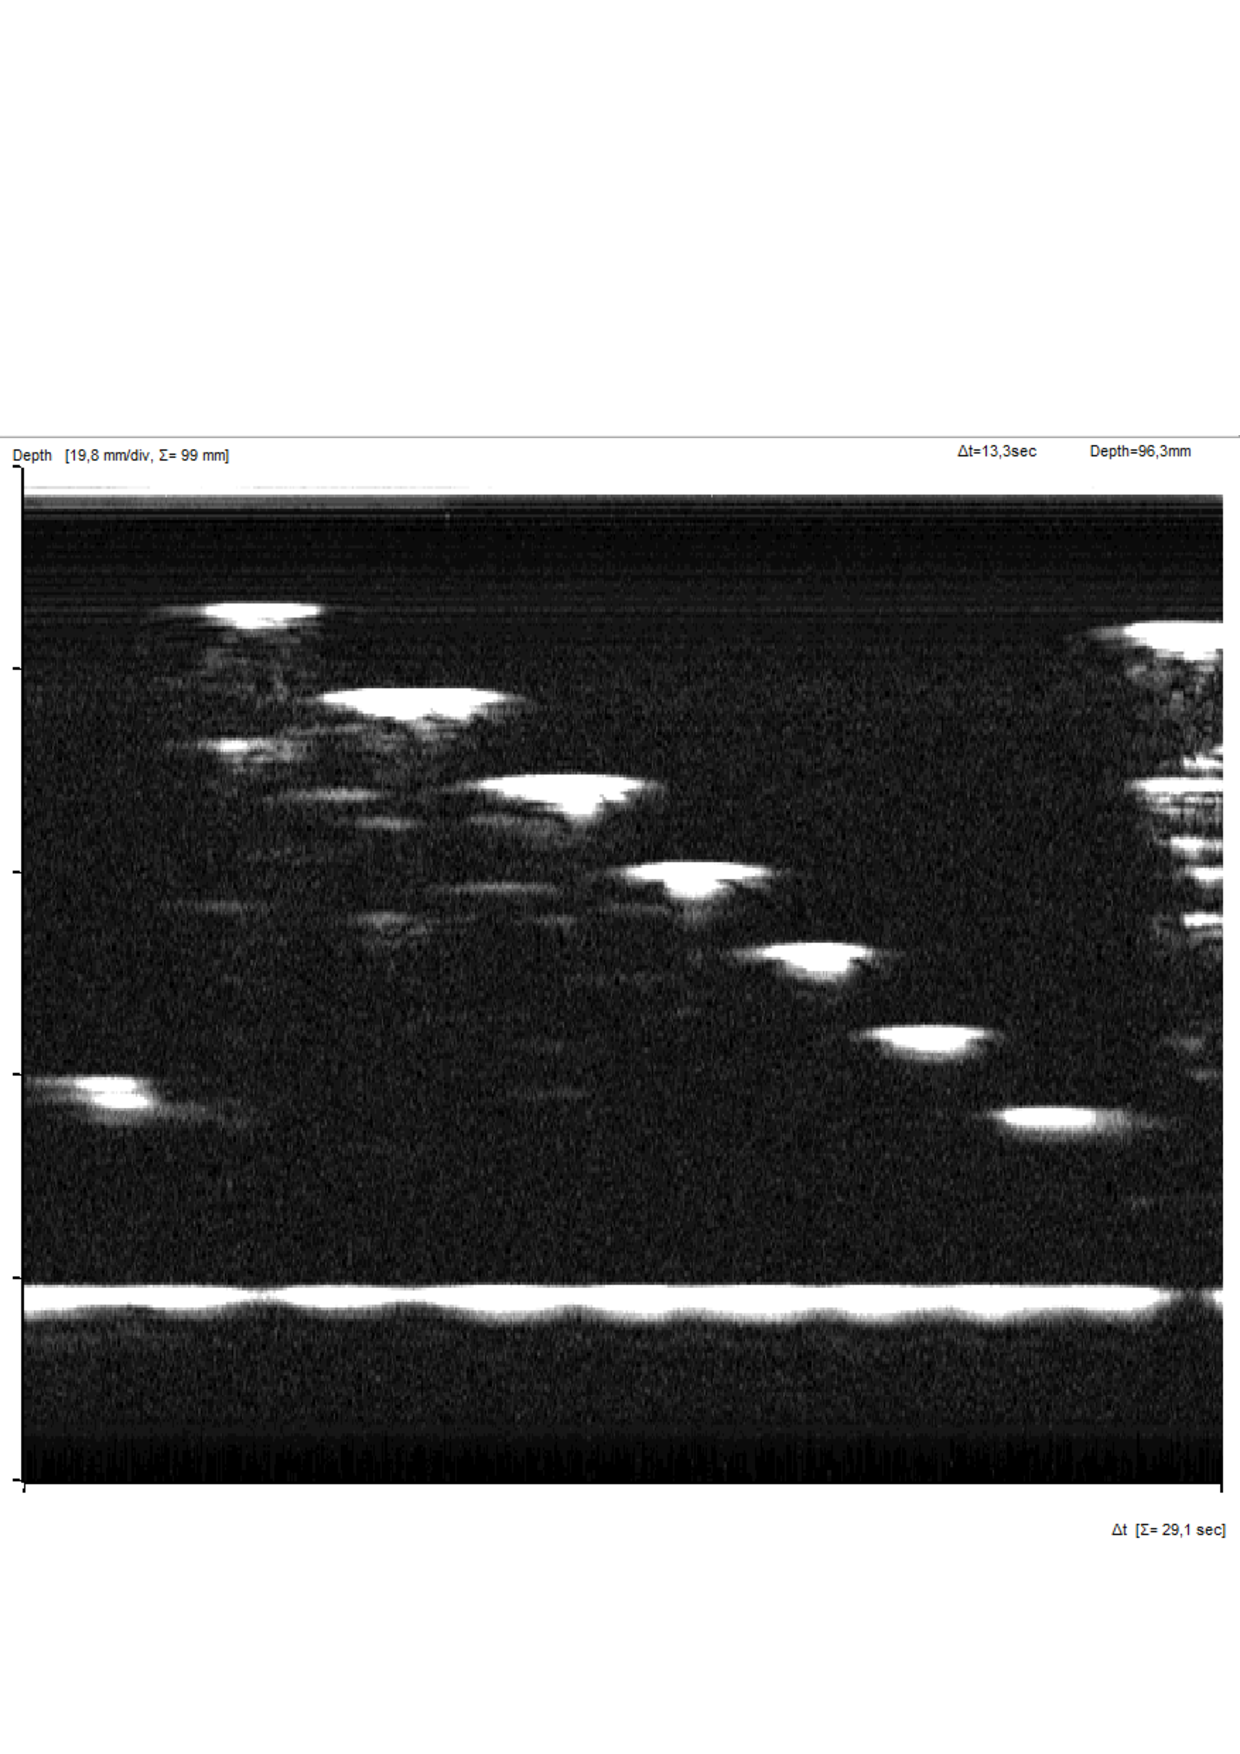
\includegraphics[height=8cm]{content/pics/B-Scan_1.pdf}
    \caption{Aufnahme des B-Scans der Oberseite des Acrylblocks.}
    \label{fig:B-Scan oben}
  \end{figure}

  \begin{figure}[H]
    \centering
    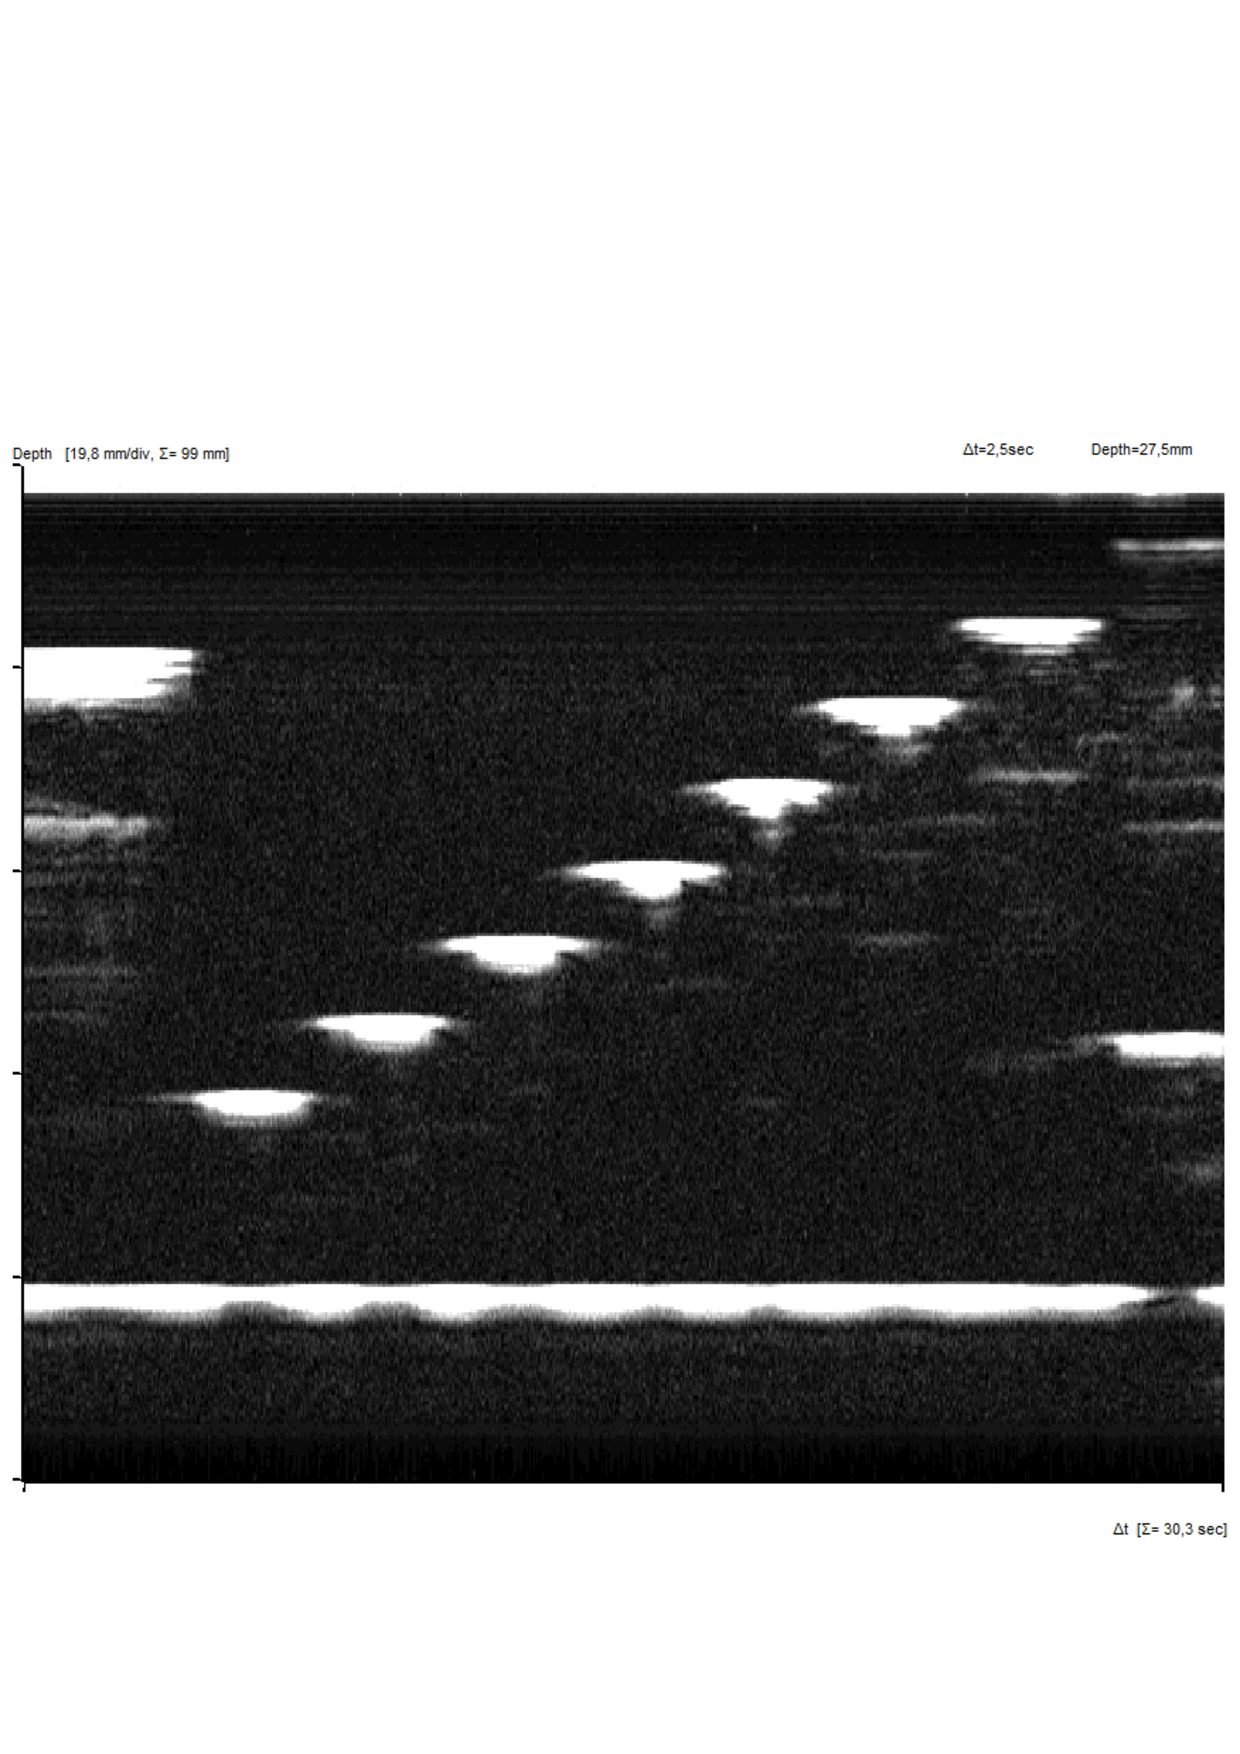
\includegraphics[height=8cm]{content/pics/B-Scan_2.pdf}
    \caption{Aufnahme des B-Scans der Unterseite des Acrylblocks.}
    \label{fig:B-Scan unten}
  \end{figure}

  \begin{table}[H]
    \centering
    \caption{Unkorrigierte Daten der Vermessung des Acrylblocks mit einem B-Scan.}
    \label{tab:b-scan}
    \begin{tabular}{S[table-format=2.0] S[table-format=2.1] S[table-format=2.1] S[table-format=2.1]}
        \toprule
         {Lochnummer} & {$\tilde{s}_{\symup{oben}}\,/\,\unit{\milli\metre}$} & {$\tilde{s}_{\symup{unten}}\,/\,\unit{\milli\metre}$} \\
        \midrule
         1	& 15.4 & 62.9 \\
         2	& 23.6 & 55.5 \\
         3	& 31.2 & 47.9 \\
         4	& 40.6 & 40.7 \\
         5	& 48.6 & 32.7 \\
         6	& 56.6 & 24.8 \\
         7	& 64.6 & 17.0 \\
         8	& {}   &  9.4 \\
         9	& 17.2 & 57.4 \\
         10	& 61.4 & 21.6 \\
         11	& 63.4 & 19.8 \\
        \bottomrule 
    \end{tabular}
  \end{table}

  Auch hier werden wie zuvor bei der Auswertung des A-Scans die Messwerte um die Dicke der Anpassungsschicht korrigiert und es wird die 
  relative Abweichung zu den Werten aus \ref{sec:Abmessungen} angegeben.

  \begin{table}[H]
    \centering
    \caption{Korrigierte Daten der Vermessung des Acrylblocks mit einem B-Scan.}
    \label{tab:b-scan_korr}
    \begin{tabular}{S[table-format=2.0] S[table-format=2.1] S[table-format=2.2] S[table-format=2.1] S[table-format=2.2]}
        \toprule
         {Lochnummer} & {$s_{\symup{oben}}\,/\,\unit{\milli\metre}$} & {$\symup{\Delta}_{\symup{rel}}(s_{\symup{oben}})\,/\,\unit{\percent}$} & %
         {$s_{\symup{unten}}\,/\,\unit{\milli\metre}$} & {$\symup{\Delta}_{\symup{rel}}(s_{\symup{unten}})\,/\,\unit{\percent}$} \\
        \midrule
         1	& 14.0 &  7.24 & 61.5 &  0.41 \\
         2	& 22.2 &  2.53 & 54.1 &  0.46 \\
         3	& 29.8 &  1.16 & 46.5 &  0.54 \\
         4	& 39.2 &  1.16 & 39.3 &  0.89 \\
         5	& 47.2 &  1.39 & 31.3 &  1.13 \\
         6	& 55.2 &  0.82 & 23.4 &  1.95 \\
         7	& 63.2 &  0.55 & 15.6 &  4.33 \\
         8	&  {}  &  {}   &  8.0 & 14.99 \\
         9	& 15.8 & 53.87 & 56.0 &  1.17 \\
         10	& 60.0 &  0.75 & 20.2 &  3.84 \\
         11	& 62.0 &  1.22 & 18.4 &  3.07 \\
        \bottomrule 
    \end{tabular}
  \end{table}
  
  
  
  
  
  
  
  
  
  
  
  
  
  
  
  
  
  
  
  
  
  
  
  
  
  
  
  
  
  
  
  
  
  
  
  
  
  
  
  
  
  



































